 \begin{frame}
    \frametitle{Teorie portfolia}
    \begin{itemize}
      \item Teorie portfolia je mikroekonomickou disciplínou, která zkoumá, jaké kombinace aktiv je vhodné držet, aby takto vytvořené portfolio mělo předem určené vlastnosti. \cite[str. 1]{camsky}
         \begin{itemize}
           \item očekávaný výnos
           \item riziko, že se skutečný výnos od očekávaného odchýlí
    \end{itemize}
    \end{itemize}
  \end{frame}
  \begin{frame}
    \frametitle{Výnosnost jako náhodná veličina}
    \begin{itemize}
      \item konečná množina aktiv $\{A_1,A_2,\dots,A_n\}$ 
      \item známe minulý vývoj
      \item ceny a výnosy v~budoucnosti neznáme
      \item na budoucí výnosnosti aktiv nahlížíme jako na náhodné veličiny
      \item stejně tak je náhodnou veličinou budoucí výnosnost celého portfolia
      \item neznáme pravděpodobnostní rozdělení těchto náhodných veličin
      \item riziko měříme pomocí směrodatné odchylky náhodné veličiny představující budoucí výnosnost aktiva
    \end{itemize}
  \end{frame}
  \begin{frame}
   \frametitle{Výnosnost portfolia}
      \begin{itemize}
        \item portfolio tvořené aktivy $A_1,A_2,\dots,A_n$
        \item váha aktiva $A_i$ v~portfoliu je $w_i$
        \item  váhy musí splňovat následující omezení:
			\begin{gather}
				\sum_{i=1}^n w_i = 1 \label{wr1}, \\
				0 \leq w_i \leq 1, \quad i\in\{1,\dots,n\}. \label{wr2}
			\end{gather}
        \item $R_i$ $\dots$ výnosnost aktiva $A_i$, $i \in \{1,\dots, n\}$
        \item $R$ výnosnost celého portfolia
        \item pak
          	\[
				R = w_1R_1+w_2R_2+\dots+w_nR_n = \sum_{i=1}^n w_iR_i.
			\]
      \end{itemize}
   \end{frame} 
   
    \begin{frame}
    \frametitle{Výnosnost portfolia a riziko }
 \begin{itemize}
\item  hodnoty výnosností aktiv neznáme $\Rightarrow$ budou nás zajímat jejich očekávané hodnoty
\item  z~linearity střední hodnoty:
\begin{equation}
E\left(\sum_{i=1}^n w_iR_i\right)=\sum_{i=1}^n w_iE(R_i). \label{ER}
\end{equation}
\item riziko měříme pomocí rozptylu, či směrodatné odchylky
\item k~výpočtu rozptylu náhodné veličiny $R$ potřebujeme kovariance náhodných veličin
\[
cov(R_i, R_j)=E\left( \left(R_i - E(R_i) \right)\left(R_j - E(R_j) \right)\right), \quad i,j \in \{1,\dots, n\}.
\]
\item Pro rozptyl náhodné veličiny $R$ platí
\[
D(R)=D\left(\sum_{i=1}^n w_iR_i\right)=\sum_{i=1}^n \sum_{j=1}^n w_iw_jcov(R_i,R_j).\
\]
\end{itemize}
    
    \end{frame}
\begin{frame}
\frametitle{Maximalizace očekávaného výnosu}
\begin{itemize}
\item  uvažme investora, který chce najít portfolio přinášející maximální očekávaný výnos
\item hledá konstanty $w_1,w_2,\dots,w_n$ splňující podmínky \eqref{wr1} a \eqref{wr2}, pro něž nabývá střední hodnota $E(R)$ maxima, tj. řeší úlohu

\small{
\begin{gather} 
\max\left\{ E\left(\sum_{i=1}^n w_iR_i\right) \bigg| \sum_{i=1}^n w_i = 1 \wedge w_i \in \mathbb{R}, 0 \leq w_i \leq 1, i\in\{1,\dots,n\} \right\}. \label{maxER}
\end{gather}}

\item řešením úlohy \eqref{maxER} je
\begin{gather*}
w_j=1,\quad j=\arg \max_{1 \leq i \leq n} E(R_i), \\
w_i=0,\quad i\in\{1,\dots,n\}, i \neq j, 
\end{gather*}
\begin{itemize}
\item  za předp., že mezi $E(R_1),E(R_2),\dots,E(R_n)$ existuje jediné maximum
\item  portfolio z~jediného aktiva - bez diverzifikace
\end{itemize}
\end{itemize}
\end{frame}

\begin{frame}
    \frametitle{Metody kvantifikace očekávaného výnosu a rizika}
    \begin{itemize}
      \item budoucí výnosnosti aktiv neznáme
      \item neznáme ani pravděpodobnostní rozdělení těchto náhodných veličin
      \item odhady charakteristik těchto náhodných veličin
      	\begin{itemize}
			\item historická metoda
			\[
\overline{r_i}=\frac{1}{T}\sum_{j=1}^T r_{ij},
\quad
s_i=\sqrt{\frac{1}{T-1}\sum_{j=1}^T (r_{ij}-\overline{r_i})^2},
\]
\[
s_{ik}=\frac{1}{T-1}\sum_{j=1}^T (r_{ij}-\overline{r_i})(r_{kj}-\overline{r_k})
\]
			\item expertní metoda
		\end{itemize}
    \end{itemize}
  \end{frame}

\begin{frame}
    \frametitle{Markowitzův model}
    \begin{itemize}
      \item Harry MARKOWITZ: \emph{Portfolio Selection.} 1952.
      \item maximalizace očekávaného výnosu portfolia a současně minimalizace rizika
      \begin{itemize}
      \item protichůdné cíle 
      \item odpor k~riziku je velmi subjektivní
       \end{itemize}
      \item o~vztahu investora k~riziku vypovídají indiferenční křivky
      \item pouze některých kombinací výnosnosti a rizika lze dosáhnout
      \item není potřeba uvažovat všechny kombinace - některé můžeme vyloučit
    \end{itemize}
  \end{frame}
  
  \begin{frame}
    \frametitle{Indiferenční křivky}
    \begin{itemize}
      \item portfolio = bod v~kartézské soustavě souřadnic
      \begin{itemize}
			\item osa $x$: riziko měřené směrodatnou odchylkou
			\item osa $y$: očekávaná výnosnost
		\end{itemize}
      \item IC - všechny kombinace portfolií, které investor považuje za stejně žádoucí
    \begin{figure}[htb]
\centering
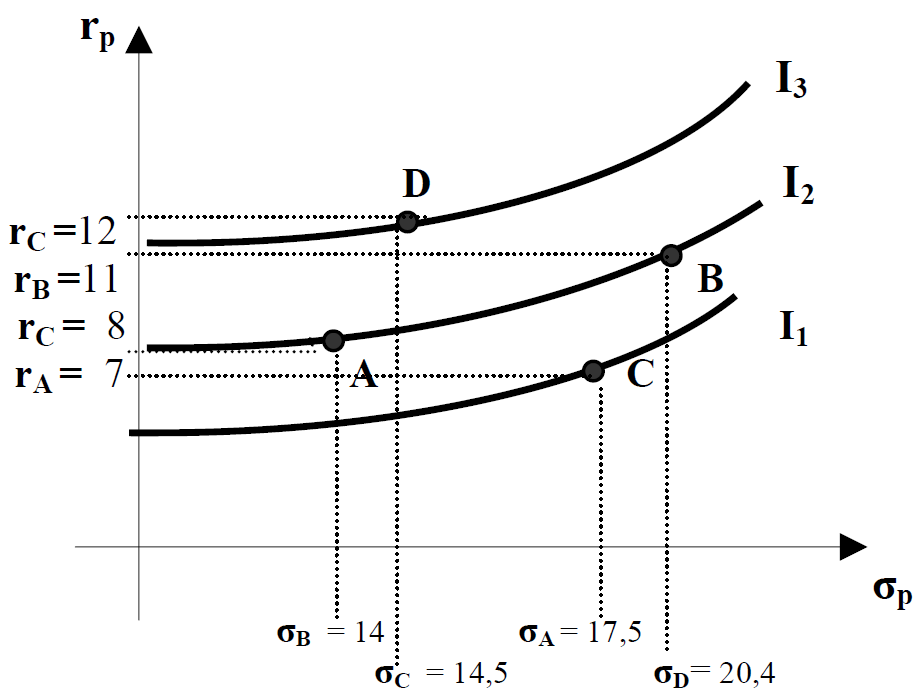
\includegraphics[width=.4\textwidth]{IC0.png}
\caption{Příklad indiferenčních křivek, zdroj: \cite{camsky} \label{obr_IC}}
\end{figure}
    \end{itemize}
  \end{frame}
  
  \begin{frame}
    \frametitle{Indiferenční křivky dle míry odporu k~riziku}
    \begin{figure}[htb]
\centering
\subfigure[Investor s~vysokým odporem k~riziku]{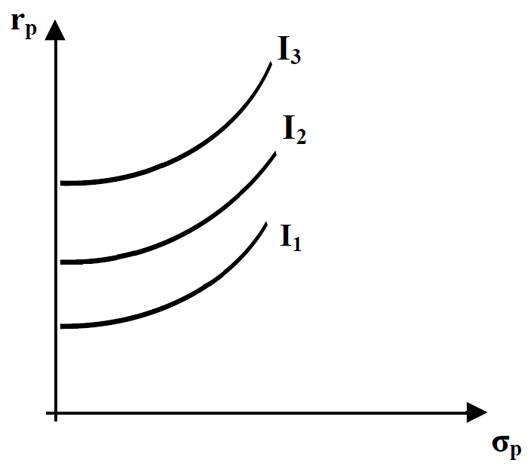
\includegraphics[width=.30\textwidth]{IC3.png}} 
\subfigure[Investor s~mírným odporem k~riziku]{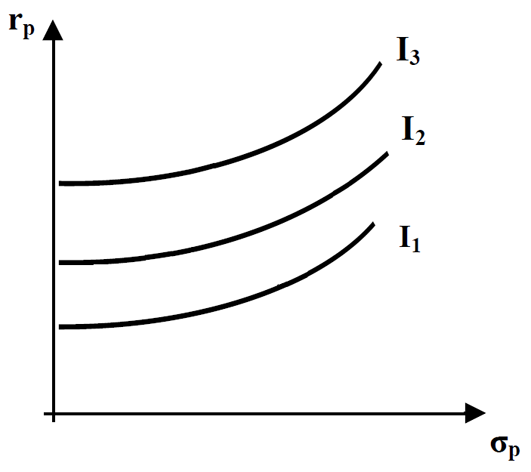
\includegraphics[width=.30\textwidth]{IC2.png}} 
\subfigure[Investor s~nepatrným odporem k~riziku]{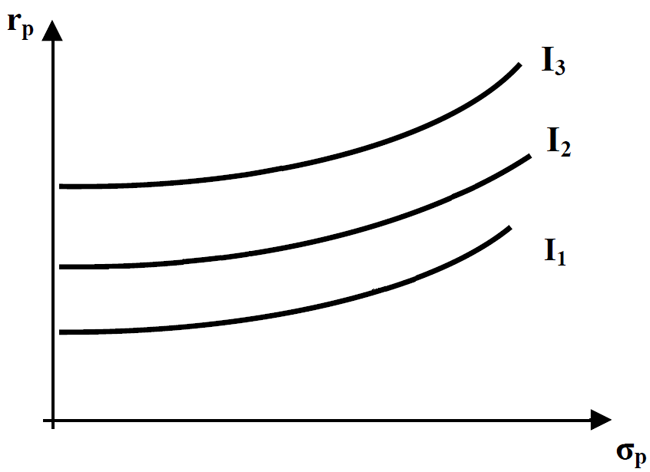
\includegraphics[width=.35\textwidth]{IC1.png}} 
\caption{Indiferenční křivky investora dle míry odporu k~riziku, zdroj: vlastní vyobrazení \label{obr_ICs}}
\end{figure}
  \end{frame}

\begin{frame}
    \frametitle{Efektivní množina}
    \begin{itemize}
      \item nekonečně mnoho portfolií
      \item \emph{přípustná množina} -  mn. všech portfolií složených z~aktiv $A_1,A_2,\dots,A_n$
      \item stačí se omezit na efektivní množinu
       \end{itemize}
       \begin{block}{Efektivní množina}
       \emph{Efektivní množina} je množina všech portfolií z~přípustné množiny, které splňují obě dvě následujících podmínky:
\begin{itemize}
\item v~přípustné množině neexistuje portfolio se stejným rizikem a vyšším očekávaným výnosem,
\item v~přípustné množině neexistuje portfolio se stejným očekávaným výnosem a nižším rizikem. 
\end{itemize}
       \end{block}
\end{frame}


\begin{frame}
    \frametitle{Efektivní množina - příklad}
    \begin{figure}[htb]
\centering
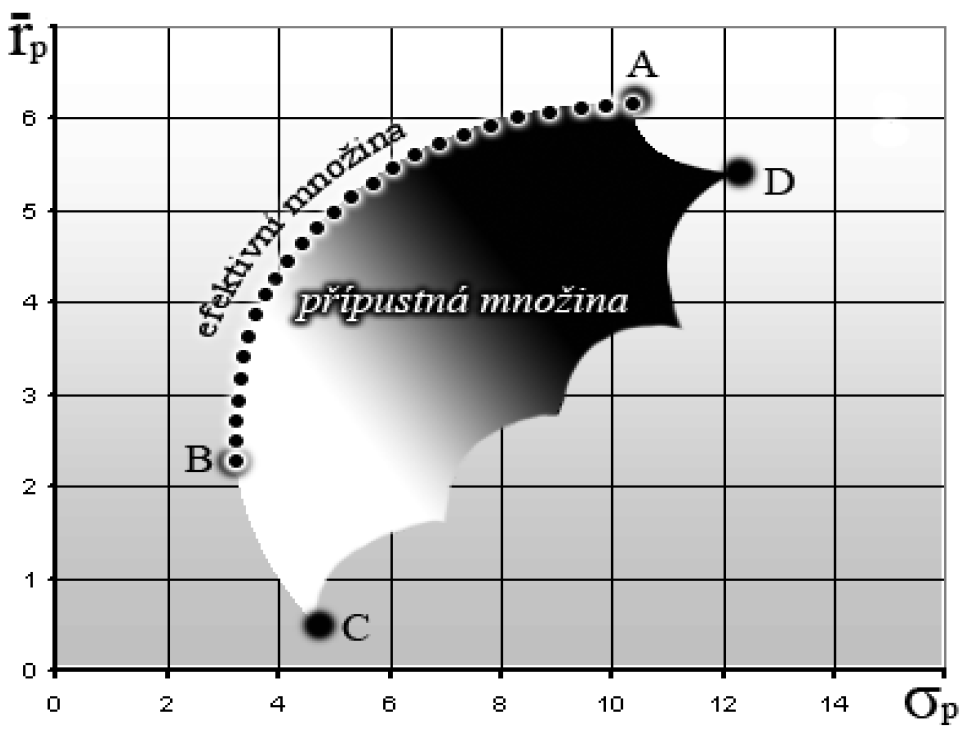
\includegraphics[width=.6\textwidth]{ef_mn.png}
\caption{Přípustná a efektivní množina, zdroj: \cite{camsky} \label{ef_mn}}
\end{figure}
  \end{frame}
  
  \begin{frame}
  \begin{itemize}
  \frametitle{Hledání efektivní množiny}
 \item Hledání efektivní množiny můžeme popsat následovně:
\begin{itemize}
\item pro každou fixní úroveň rizika nalezneme všechna dostupná portfolia s~maximální očekávanou výnosností, 
\item pro každou fixní úroveň očekávané výnosností nalezneme všechna dostupná portfolia s~minimálním rizikem,
\item do efektivní množiny zařadíme právě ta portfolia, která byla vybrána v~obou předchozích krocích.
\end{itemize}
\end{itemize}
  \end{frame}
  
  

\begin{frame}
    \frametitle{Výběr optimálního portfolia}
    \begin{itemize}
      \item výběr z efektivní množiny na základě indiferenčních křivek
      \item investor vybere portfolio z~efektivní množiny ležící na nejvyšší indiferenční křivce

\begin{figure}[htb]
\centering
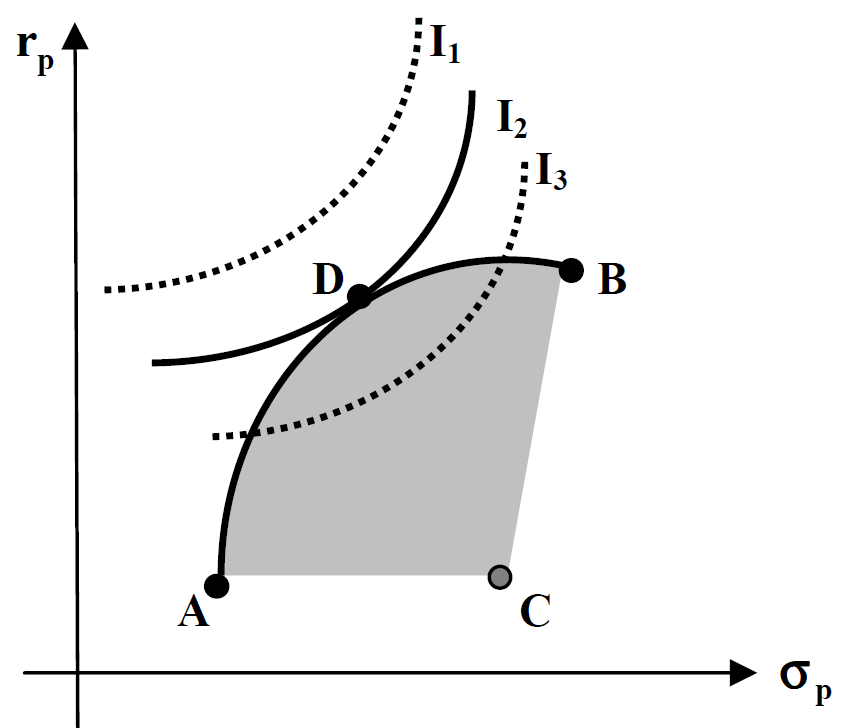
\includegraphics[width=.4\textwidth]{vyber.png}
\caption{Výběr optimálního portfolia, zdroj: \cite{camsky} \label{vyber}}
\end{figure}
    \end{itemize}
  \end{frame}

